\documentclass[11pt,a4paper]{article}
\usepackage{ctex}
\usepackage[utf8]{inputenc}
\usepackage{geometry}
\usepackage{fancyhdr}
\usepackage{enumitem}
\usepackage{titlesec}
\usepackage{amsmath} % Added for math equation support
\usepackage{graphicx} % Added for including graphics
\usepackage{titling}
\usepackage{subcaption}

\usepackage{multicol}
\usepackage{listings}
\usepackage{booktabs}
\usepackage{multirow}

\usepackage[hidelinks]{hyperref}
% \usepackage[style=authoryear]{biblatex} % Use biber backend
% \addbibresource{../../paper.bib} % Specify the .bib file
% Define \lll
\newcommand{\lll}{\mathrel{<\!\!<\!\!<}}
% Define \ggg
\newcommand{\ggg}{\mathrel{>\!\!>\!\!>}}
\geometry{margin=0.5in}
\titleformat{\section}{\large\bfseries}{\thesection}{0.5em}{}

% title context and style setting
\title{周报-向嘉豪(2024-11-25)}
\setlength{\droptitle}{-6em} % Reduce space begin the title
% Redefine \maketitle to display only the title
\renewcommand{\maketitle}{
  \begin{center}
    \LARGE\bfseries\thetitle
  \end{center}
}

\begin{document}

\maketitle


% Custom Abstract
\noindent \textbf{Abstract}: 本周工作取得三项主要进展:1)完成LCB基准测试框架的跨平台扩展,成功将ESP32S3纳入测试平台族群,并通过QARMAv2算法的性能评测验证了框架的可扩展性;2)论文撰写达到初稿水平,重点完善了算法优化实现方法、实验结果分析以及结论展望等核心章节,经查重系统检测,相似度为9\%,符合学术规范;3)基于IEEE期刊推荐系统的分析结果,优选出4个潜在目标期刊,其中IEEE Transactions on Information Forensics and Security(IF=6.3)因其研究方向契合度高且影响因子显著,确定为首选投稿目标。

\noindent \textbf{下周计划}: 1)对论文进行精细化修订;2)按IEEE期刊模版重构论文格式。

\subsection{LCB框架跨平台扩展}
为验证LCB基准测试框架的跨平台通用性,本周成功将支持平台扩展至ESP32S3。通过在该平台上对QARMAv2加密算法进行系统性能评测,发现相同实现在ESP32S3上的执行效率较基准平台降低约50\%,这一结果有力证实了硬件平台特性对加密算法性能的显著影响。

\subsection{论文核心内容完善}
本周重点完善了论文的三个关键章节:第4.1节详细阐述了AES算法的优化实现方法论;第4.3节系统呈现了实验环境配置、性能测试结果及其对比分析;第5章总结了研究成果并提出未来优化方向。论文初稿经查重系统检测(如图\ref{fig:check}所示),相似度为9\%,表明内容具有良好的创新性。

\begin{figure}[h]
  \centering
  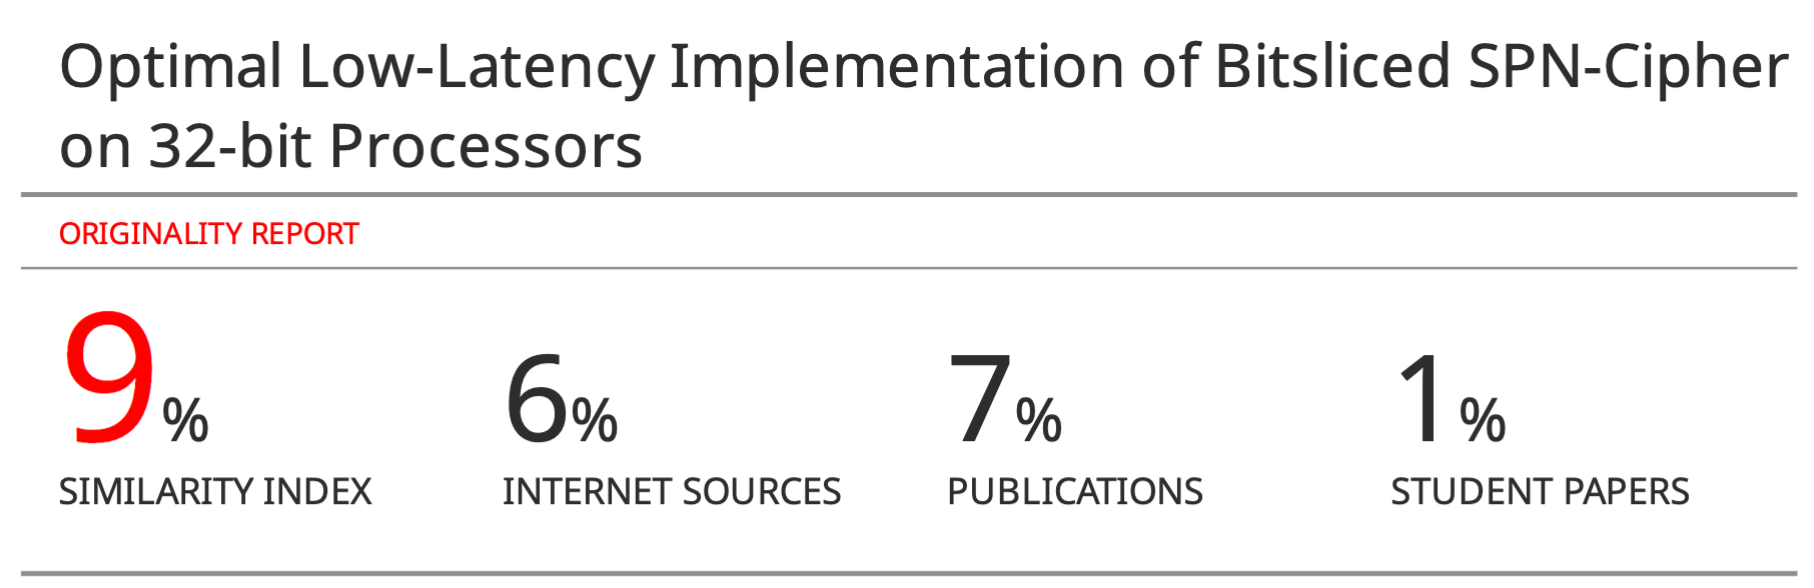
\includegraphics[width=0.5\textwidth]{./fig/duplicate_9.png}
  \caption{查重结果}
  \label{fig:check}
\end{figure}

\subsection{目标期刊甄选}
基于IEEE期刊推荐系统(\url{https://publication-recommender.ieee.org}),通过输入研究摘要获取了20个相关Trans期刊。经过对影响因子、审稿周期、期刊定位等多维度分析,筛选出4个候选期刊(详见表\ref{tab:journal})。考虑到IEEE Transactions on Information Forensics and Security在2022年发表过相近研究主题的文章,且具备最高影响因子(6.3)和较优审稿周期(5个月),将其确定为首选投稿目标。


\begin{table}[ht]
    \centering
    \caption{目标期刊对比分析}
    \label{tab:journal}
    \begin{tabular}{lcccc}
        \toprule
        期刊名称 & 分区 & IF值 & 审稿周期(月) &年文章数 \\
        \midrule
        IEEE Trans. on Consumer Electronics & 2区 & 4.3 & 3 & 224 \\
        IEEE Trans. on Industry Applications & 2区 & 4.2 & 3 & 769 \\
        \textbf{IEEE Trans. on Info. Forensics and Security} & 1区/CCF-A & 6.3 & 5 & 799 \\
        IEEE Trans. on Computers & 2区/CCF-A & 3.6 & 6 & 144 \\
        \bottomrule
    \end{tabular}
    \small
    \caption*{年文章数:为该期刊2024发表的文章数。 审稿周期:查看最新一期的文章,计算从投稿到发表的时间,三篇取平均值。}
\end{table}

% \newpage
% % Add some vertical space to push content to bottom if needed
% \vfill


% % Include the bibliography
% \bibliographystyle{alpha}
% \bibliography{../../paper}

\end{document}